% SWOTxAI manuscript scaffold. Written 2026-11-14, reduced to an outline 2026-11-15 (research plan Phase 3 target: JGR Oceans).
% Build: bash papers/manuscript/build.sh main
% Convention: no drafted prose. Every red bracketed bullet is a note on what the paragraph should
% say (facts, numbers, citations); David writes the sentences. \todo marks an open decision.
% \fig points at a figure that already exists under docs/figures/ (the paths resolve from this folder).
% Switch \documentclass to AGU's agujournal2019 before submission; the section plan is AGU's.
\documentclass[11pt]{article}
\usepackage[margin=1in]{geometry}
\usepackage{amsmath,amssymb,booktabs,array,graphicx,xcolor,hyperref,natbib}
\usepackage[T1]{fontenc}
\graphicspath{{../../docs/figures/}}
\definecolor{note}{named}{red}
\colorlet{note}{red!70!black}
\newcommand{\todo}[1]{\textcolor{note}{[\textbf{TODO} #1]}}
\newcommand{\fig}[1]{\texttt{docs/figures/#1}}
\newcommand{\R}{R^2}
% notes: a red bracketed bullet list; \nb{...} is one note. Equations inside a note stay black.
\newenvironment{notes}{\begin{itemize}\color{note}}{\end{itemize}}
\newcommand{\nb}[1]{\item\relax[#1]}
\newenvironment{eqblack}{\begingroup\color{black}}{\endgroup}
\bibliographystyle{plainnat}  % use agufull08 once the AGU class is in place

\title{\todo{title. Working: ``Hourly surface currents from a single SWOT pass: a radar-validated model with wind history, nineteen coastal networks, two held-out years''}}
\author{David A. Lee$^{1}$ \and \todo{co-authors and advisor}\\[4pt]
\small $^{1}$Columbia University}
\date{Outline of 15 November 2026}

\begin{document}
\maketitle

\section*{Key Points}
\begin{notes}
  \nb{Key point 1, time transfer: trained on year one of SWOT, no measurable drift over two further years on nineteen radar networks; no transfer to networks not seen in training.}
  \nb{Key point 2, the hourly result: with the wind at the target hour and its two-day history, one pass predicts the hourly surface current with no loss of skill out to twelve hours either side.}
  \nb{Key point 3, the daily-target negative: on the 25-hour-mean current the same wind history adds nothing; the averaged target removes the inertial motion that carries it.}
  \nb{AGU limit: 140 characters each.}
\end{notes}

\begin{abstract}
\begin{notes}
  \nb{250 words.}
  \nb{What SWOT gives: sea surface height over a 120-km swath once every few days; the implied current is geostrophic, instantaneous, sparse in time.}
  \nb{What we train: one model on SWOT Level-3 height and geostrophy, ERA5 wind, mean dynamic topography.}
  \nb{Truth: HF radar surface currents, nineteen coastal networks, three continents.}
  \nb{Protocol: hold out time (train cycles 001--016, score 017--058) and region.}
  \nb{Result 1: in time the model holds; in space only where the training set covers the regime.}
  \nb{Result 2: wind history on the 25-hour-mean target is a clean negative with a physical response function, 1.2\,\% of wind speed at 30--40$^\circ$ right.}
  \nb{Result 3: detided hourly target at offsets around each pass, wind history at the target hour and a slab-layer inertial current as inputs: skill flat across $\pm12$ h where the snapshot decays; the averaged hourly prediction beats the daily model on the daily target (uswc $u$ 0.39 against 0.35, intervals apart; no cell loses).}
\end{notes}
\end{abstract}

\section*{Plain Language Summary}
\begin{notes}
  \nb{Write last. Audience: knows what a satellite and a current are.}
  \nb{Story: a satellite photograph of the sea surface gives the current at the moment of the photograph; the wind tells how it changed since; together they give the current at any hour of that day.}
\end{notes}

\section{Introduction}
\begin{notes}
  \nb{Six paragraphs, one claim each.}
  \nb{1. What SWOT measures and why the implied current is incomplete \citep{fu2024swot,dibarboure2025l3}: geostrophy only, one snapshot per pass, balanced/unbalanced partition at small scales \citep{torres2018partition,qiu2018transition}.}
  \nb{2. What the field has done: OSSE-based learning \citep{sinha2021ml}, global eddy reconstruction \citep{martin2024eddies}, SWOT geostrophy against radar \citep{tchonang2026swot}, wind-to-current response from drifters \citep{ubelmann2025wind,elipot2016hourly}.}
  \nb{3. The gap: no model validated against independent hourly truth across continents with a temporal holdout; the leakage finding of 2026-07-21 (research log; cite in the SI).}
  \nb{4. HF radar as truth: top-metre Eulerian current plus a fraction of the Stokes drift \citep{stewart1974hfr,rohrs2015hfr}; the 25-hour mean as the field's standard target and what it hides.}
  \nb{5. This paper: the protocol, the three results (time transfer, no space transfer, the hourly result), the scoped novelty claim: first multi-region, temporally held-out, radar-validated hourly surface-current model from single-pass SWOT.}
  \nb{6. Roadmap.}
\end{notes}

\section{Data}
\subsection{SWOT Level-3 sea surface height and geostrophy}
\begin{notes}
  \nb{L3 LR SSH Expert v3.0; science orbit cycles 001--058 (July 2023 to October 2026).}
  \nb{Regridding to the radar grid; filtered geostrophy.}
  \nb{Which cycles are reprocessed and which forward-stream; disclosure list from \texttt{papers/NOTES.md}.}
\end{notes}
\subsection{High-frequency radar}
\begin{notes}
  \nb{Nineteen networks: six US (NCEI RTV archive), six European (EU HFR node), seven Australian (IMOS ACORN).}
  \nb{Grids, QC flags, record lengths; the hourly archives on which both the 25-hour and the hourly targets are built.}
  \nb{Table: region, network, spacing, record, colocated passes.}
\end{notes}
\subsection{Wind, reference products}
\begin{notes}
  \nb{ERA5 10-m wind \citep{hersbach2020era5}, hourly, July 2023 to August 2026.}
  \nb{DUACS L4 as the operational reference; MDT.}
\end{notes}

\section{Methods}
\subsection{Rows, targets and the evaluation protocol}
\begin{notes}
  \nb{Single-sourced methods text with the equations lives in \texttt{docs/methods-equations/methods-equations.tex}; \texttt{build.sh} extracts its body to \texttt{methods-baselines-body.tex}. Restore the line below once the wording is yours; trim ``Notation'' and the truth-tier section to the paper's needs.}
\end{notes}
% \begingroup\let\section\subsubsection \input{methods-baselines-body} \endgroup

\subsection{Temporal and regional holdout}
\begin{notes}
  \nb{Every model fitted on cycles 001--016 (July 2023 to June 2024), scored on 017--058 (June 2024 to August 2026).}
  \nb{Regional transfer: train on one continent, score the others; leave-one-region-out within the United States.}
  \nb{Intervals: block bootstrap over passes \citep{kunsch1989block}.}
  \nb{Refit after selection: the champion is a recipe retrained from scratch on year one, never the weights of the search.}
\end{notes}

\subsection{The learned model}
\begin{notes}
  \nb{The evolved champion: 72-column stencil, engineered block, convolutional path over the $3\times3$ stencil, MLP member, masked squared error, early stopping, no coordinates as inputs.}
  \nb{One paragraph on the evolutionary search: an audit trail, not a replicable step.}
  \nb{Trees (LightGBM) as the second learner.}
\end{notes}

\subsection{Wind history on the 25-hour target}
\begin{notes}
  \nb{Inputs: lagged ERA5 winds at pass time minus $\ell \in \{3,6,12,18,24,48,96,192\}$ h, the Coriolis parameter, the season, as extra columns on the frozen rows.}
  \nb{Response function: finite-difference Jacobian of the trained network, resolved along and across the wind direction of the row, summed over lags for the steady response:}
  \begin{eqblack}
  \begin{equation}
  \mathbf{G}_\ell = \frac{1}{N}\sum_{i=1}^{N} \frac{f_\theta(\mathbf{x}_i + \delta\,\mathbf{e}_{\ell}) - f_\theta(\mathbf{x}_i)}{\delta}, \qquad \delta = 2\ \mathrm{m\,s^{-1}}.
  \label{eq:response}
  \end{equation}
  \end{eqblack}
\end{notes}

\subsection{The hourly target and the 25 rows per pass}
\begin{notes}
  \nb{Detiding: per radar cell, least-squares fit of the training-year hourly record to five constituents; fitted sinusoids (without $a_0$) subtracted from every hour, training and test alike; cells with fewer than 2000 valid training hours not fitted and dropped from the hourly target:}
  \begin{eqblack}
  \begin{equation}
  u(t) = a_0 + \sum_{k=1}^{5}\big[a_k \cos(2\pi t/T_k) + b_k \sin(2\pi t/T_k)\big],
  \qquad T_k \in \{\mathrm{M_2, S_2, N_2, K_1, O_1}\}.
  \label{eq:harmonic}
  \end{equation}
  \end{eqblack}
  \nb{Removed variance fraction per region: 2--4\,\% US West Coast, 7--8\,\% East and Gulf.}
  \nb{Rows: each base row (cell $c$, pass time $t$) gives targets at $t + k$, $k \in \{-12, -9, \dots, +12\}$ h; SWOT stencil is the pass-time stencil; $k$ is an input; wind columns are ERA5 at $t + k - \ell$, $\ell \in \{0, 3, \dots, 24, 36, 48\}$ h; offsets $k \ne 0$ drawn for one base row in eight.}
  \nb{Split by cycle, bootstrap blocks are passes, so the rows of a pass never straddle the split.}
  \nb{Slab-layer current: Pollard--Millard slab \citep{pollard1970slab} of depth $H$ driven by ERA5 stress, integrated exactly over each hour, supplies the inertial phase as two input columns:}
  \begin{eqblack}
  \begin{equation}
  \frac{dZ}{dt} + (r + \mathrm{i} f)\,Z = \frac{\tau}{\rho H}, \qquad Z = u + \mathrm{i}v, \qquad
  \tau = \rho_a C_D |\mathbf{W}|\,\mathbf{W},
  \label{eq:slab}
  \end{equation}
  \begin{equation}
  Z_{n+1} = Z_n e^{-a\Delta t} + \frac{1 - e^{-a\Delta t}}{a\,\rho H}\,\tau_n, \qquad a = r + \mathrm{i}f,
  \label{eq:slabstep}
  \end{equation}
  \end{eqblack}
  \nb{Constants: $H = 25$ m, $r^{-1} = 4$ d, $C_D = 1.2\times10^{-3}$, $\rho = 1025$, $\rho_a = 1.22$ kg\,m$^{-3}$.}
  \nb{Seeds: 42, 43, 44 for the wind models; tables report the mean prediction; single-seed spread $\pm0.005$.}
  \nb{Sensitivity to $H$ still owed; mixed-layer climatology \citep{deboyer2004mld} as the obvious upgrade.}
\end{notes}

\section{Results}
\subsection{Transfer in time}
\begin{notes}
  \nb{Figures: \fig{holdout/skill\_through\_time\_quarterly}, \fig{holdout/transfer\_grid}.}
  \nb{Table: $\R$ per region for calibrated geostrophy, DUACS + wind, own-continent champion, all-19 champion.}
  \nb{Drift slopes with intervals: 13 of 16 regions indistinguishable from zero.}
\end{notes}
\begin{center}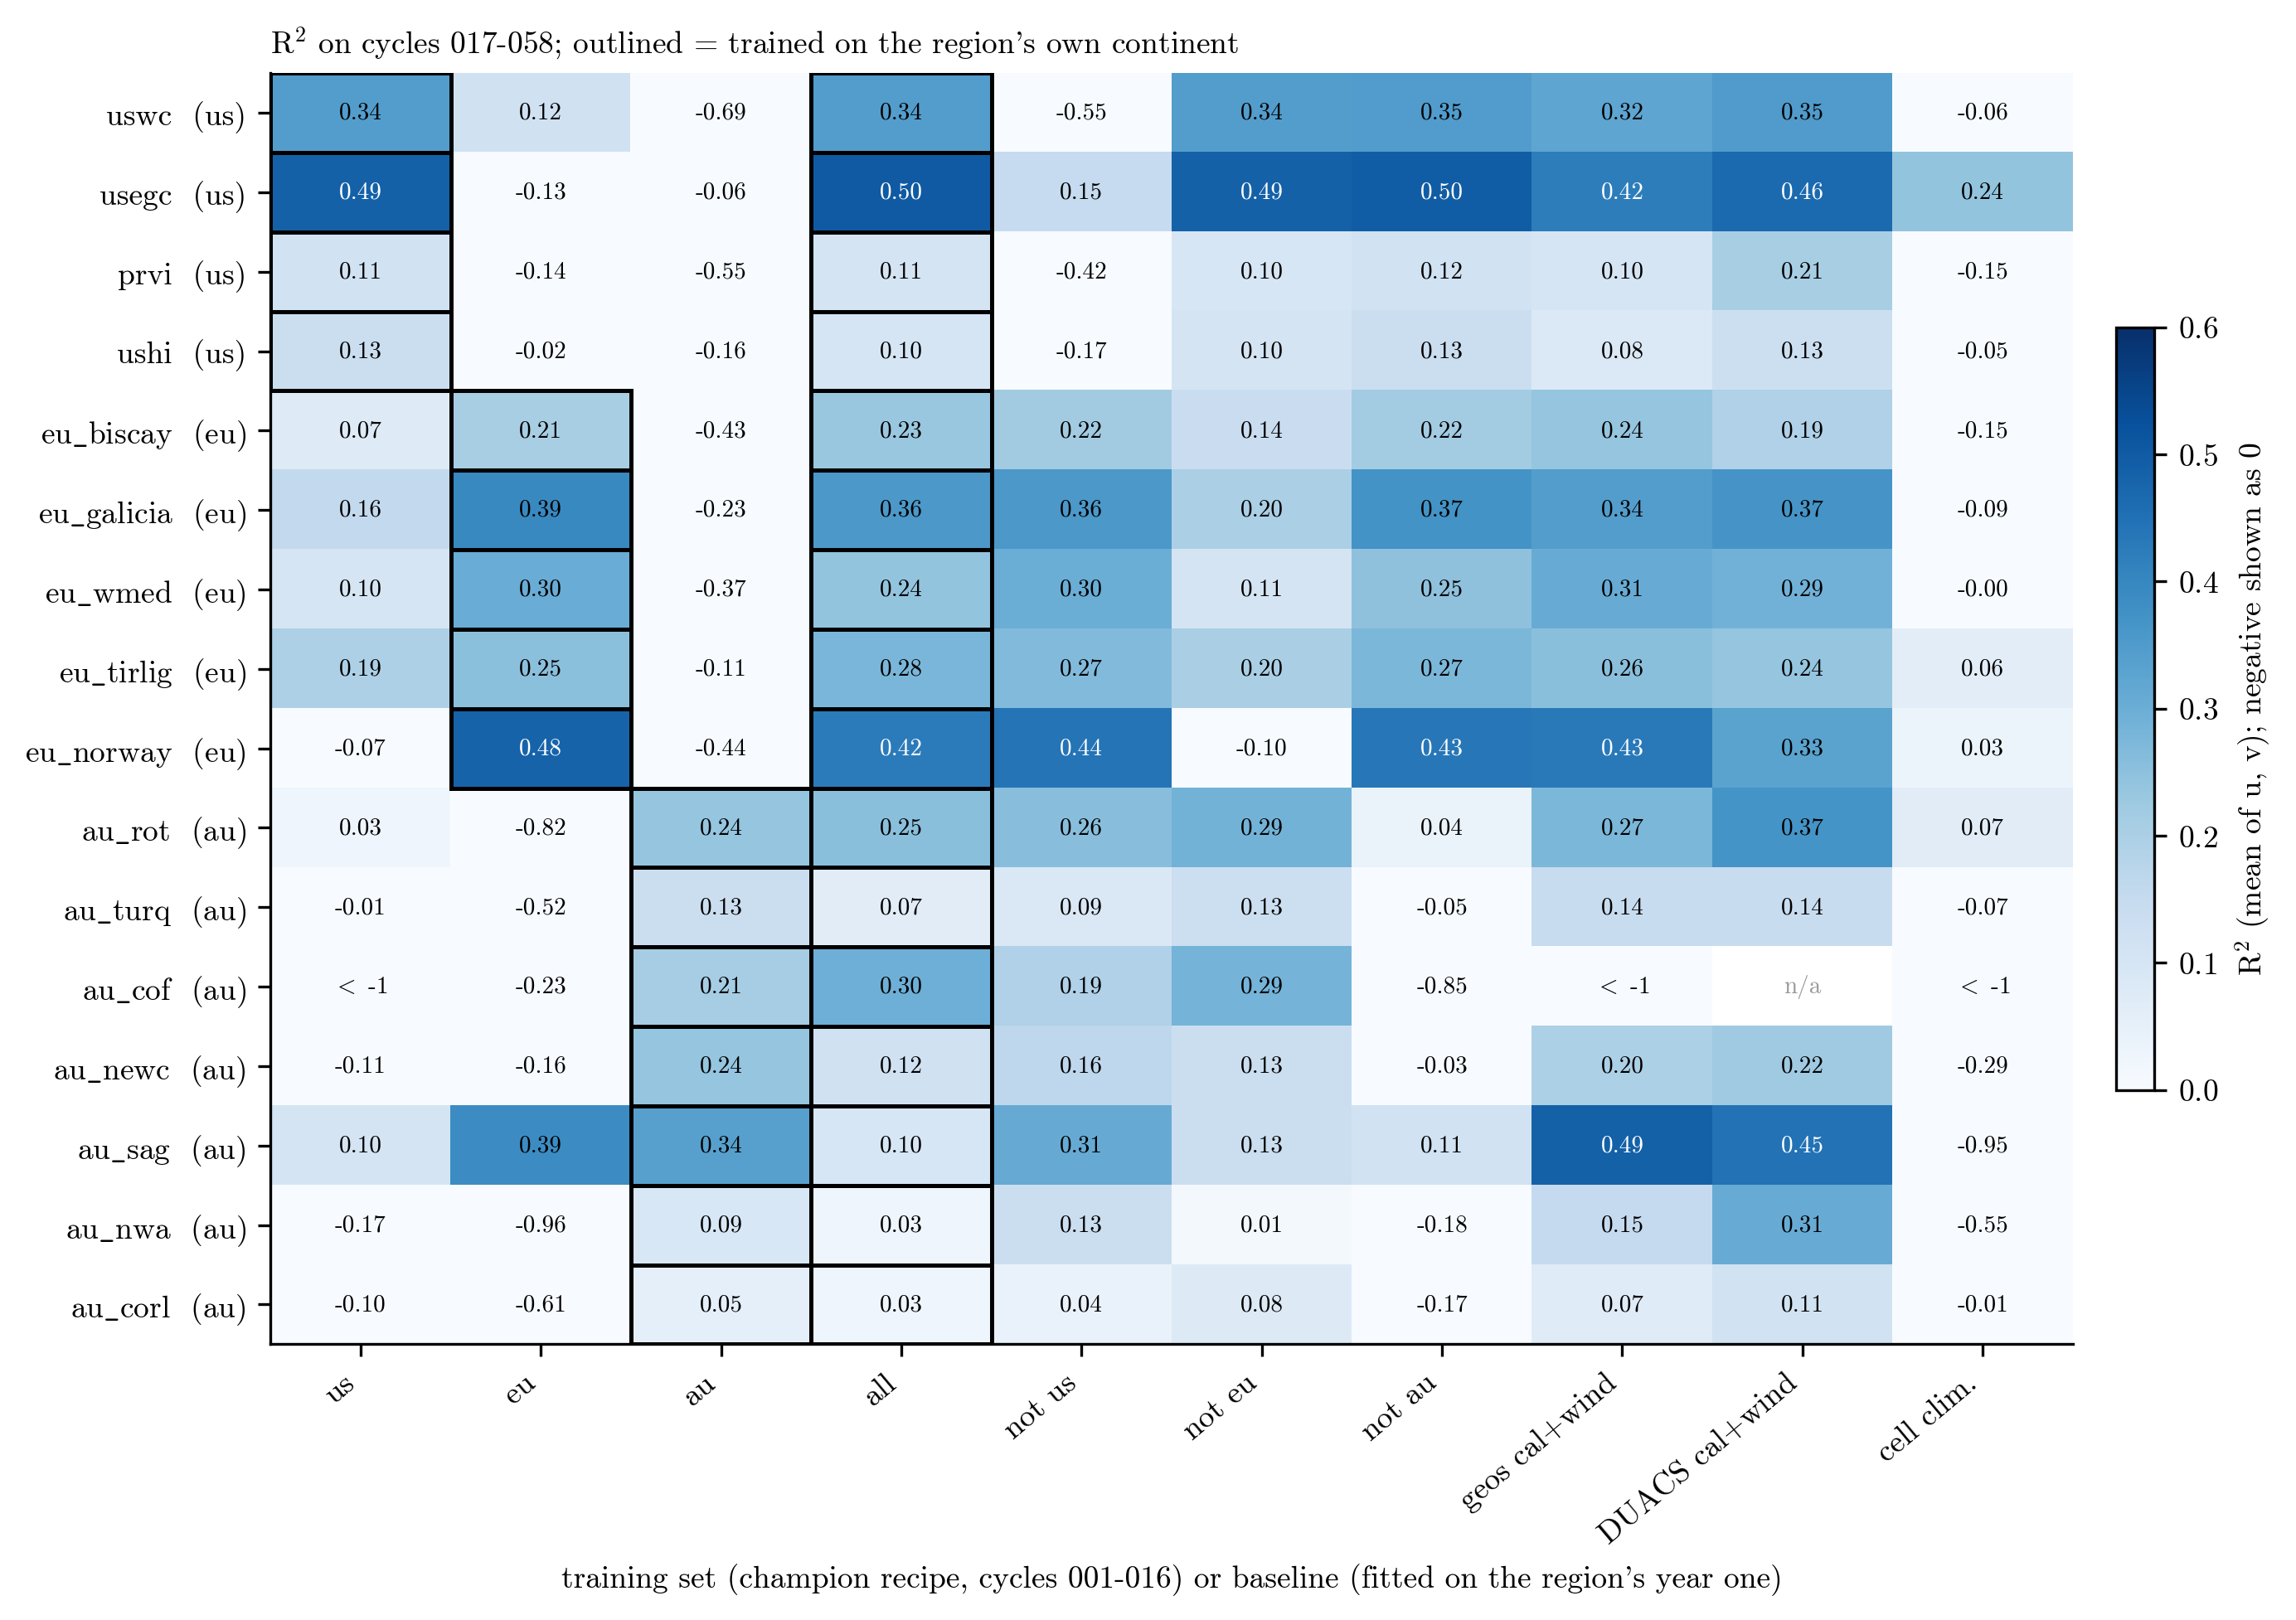
\includegraphics[width=\textwidth]{holdout/transfer_grid.png}\end{center}
\subsection{Transfer in space}
\begin{notes}
  \nb{Figures: \fig{holdout/loro\_us}, \fig{holdout/transfer\_map}.}
  \nb{Leave-one-continent-out and leave-one-region-out: $u$ collapses, $v$ survives; worse than calibrated geostrophy.}
  \nb{The Coriolis input does not rescue it; the all-19 model recovers in-region skill.}
  \nb{State the withdrawn claim plainly: train on every network you intend to predict.}
\end{notes}
\subsection{Wind history on the daily target: a clean negative with a physical response}
\begin{notes}
  \nb{Figures: \fig{holdout/wind\_history\_gain}, \fig{holdout/wind\_response}.}
  \nb{Ladder table: lags, $f$, season add nothing inside the intervals.}
  \nb{Response: 1.2\,\% of wind speed at 28--41$^\circ$ right, 70--80\,\% instantaneous; least-squares fit on the same rows agrees (1.1\,\% at 40$^\circ$, 0.9\,\% at 37$^\circ$); trees control.}
\end{notes}
\subsection{The hourly target}
\begin{notes}
  \nb{Figures: \fig{holdout/hourly\_skill\_offset}, \fig{holdout/hourly\_tide\_effect}, \fig{holdout/hourly\_wind\_response}.}
  \nb{Skill against offset for the four models: offset-only decays (uswc $u$ 0.19 at 0 h to 0.14 at $\pm12$ h), wind-lag model flat (0.28--0.30 / 0.36--0.38 uswc, 0.50--0.53 / 0.43--0.45 usegc).}
  \nb{$f$ and season: $+0.01$, same size as the three-seed ensembling gain, null.}
  \nb{Tide control: raw target loses 0.02 (uswc) and 0.11 in $u$ (usegc), matching the removed variance fractions.}
  \nb{Hourly response: 1.31\,\% at 25$^\circ$ right (uswc), 1.53\,\% at 18$^\circ$ (usegc); cross-wind response rotates clockwise through one inertial period (right at 0--3 h, left at 15--18 h, right by 24 h).}
  \nb{Averaged hourly prediction against the daily champion, three seeds both sides: uswc 0.391 / 0.557 against 0.346 / 0.522; usegc 0.701 / 0.648 against 0.694 / 0.612; no cell loses.}
  \nb{Pass-hour prediction alone against the daily mean: $u$ 0.14 uswc, 0.64 usegc; the coastal contrast in sub-daily variance, beside the rotary spectra.}
\end{notes}
\begin{center}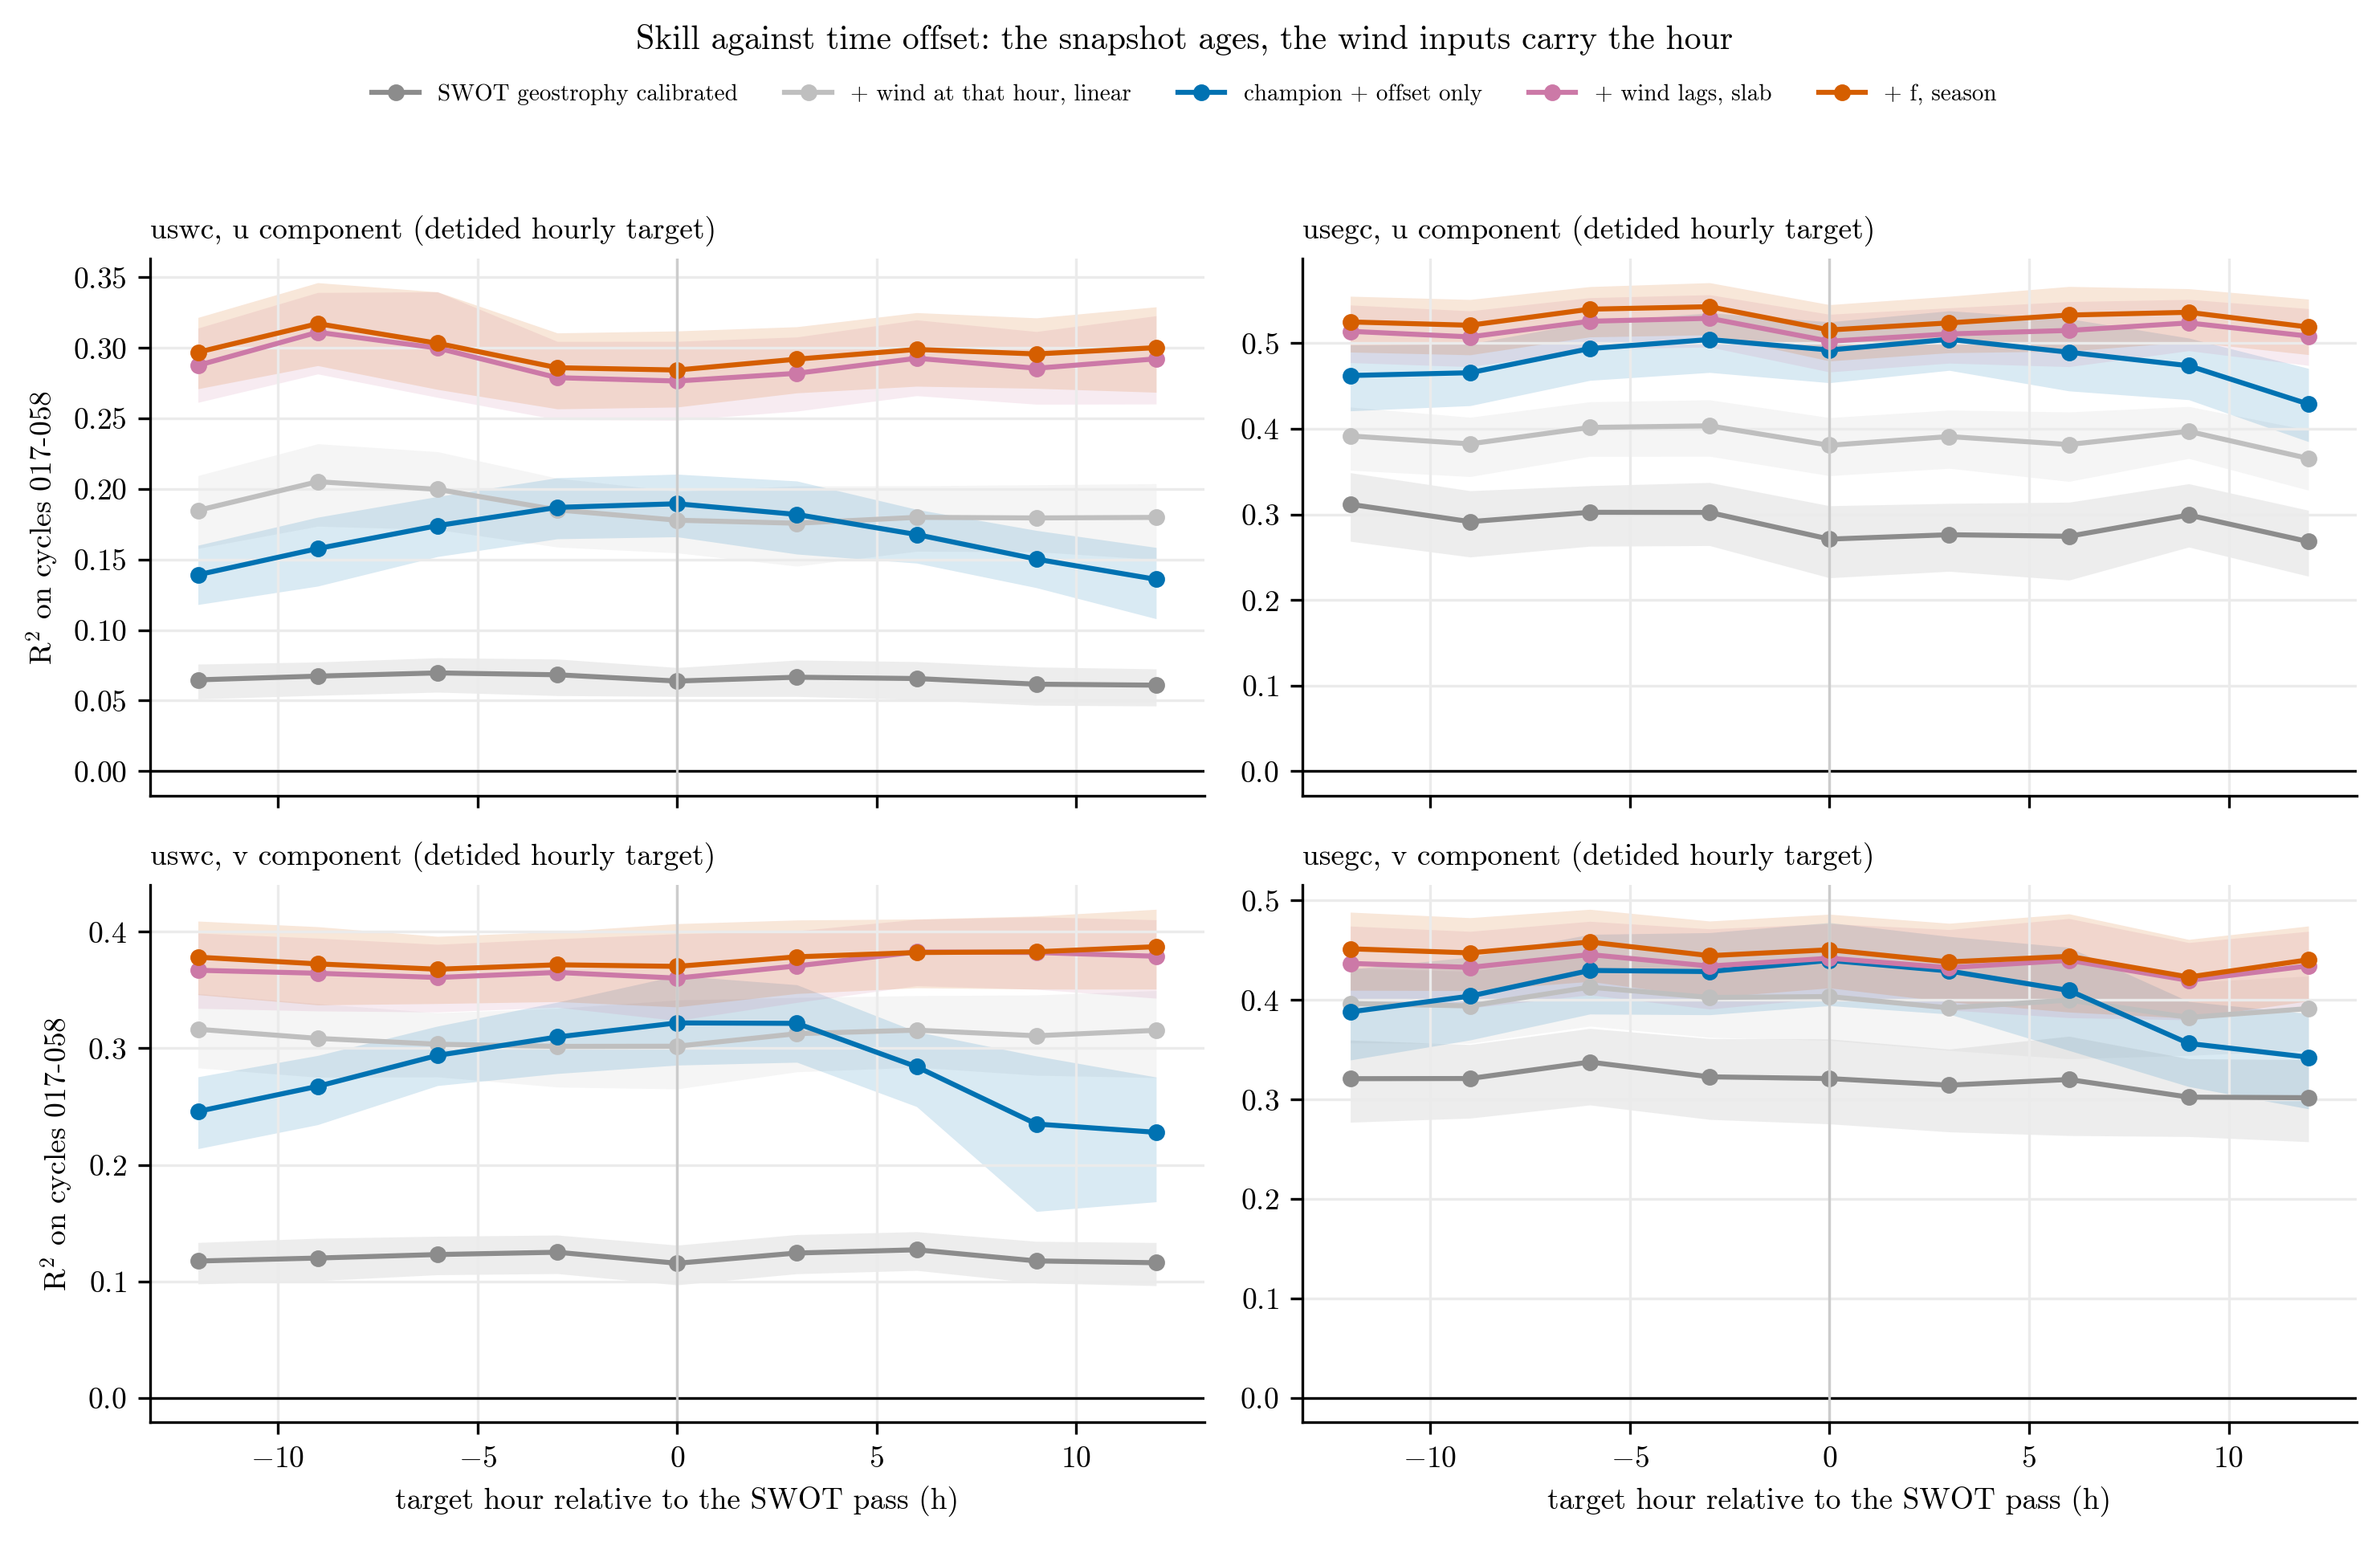
\includegraphics[width=\textwidth]{holdout/hourly_skill_offset.png}\end{center}

\section{Discussion}
\begin{notes}
  \nb{Why the 25-hour mean hides the wind: the boxcar's first null at 0.96 cpd sits on the inertial band at these latitudes; rotary spectrum figure \fig{hfr\_target/}; \citep{alford2016nio}.}
  \nb{What the radar measures against what a drifter measures \citep{rohrs2015hfr,ardhuin2009stokes}; why the response is weaker than the drifter literature \citep{ubelmann2025wind,elipot2016hourly,rio2014ekman}.}
  \nb{Shelf dynamics the stencil cannot see \citep{lentz2012innershelf,brink1991ctw}.}
  \nb{Why regional transfer fails: regime, not rotation; coverage, not capacity.}
  \nb{Toward a whole-ocean hourly product: drifters as open-ocean truth, OSSE with LLC4320, the inertial/diurnal degeneracy near 30$^\circ$.}
  \nb{Limitations: one learner family, ERA5 at 0.25$^\circ$, five tidal constituents \citep{pawlowicz2002ttide}, the radar's own error, two networks in the hourly experiment.}
\end{notes}

\section{Conclusions}
\begin{notes}
  \nb{Three sentences, one per key point.}
\end{notes}

\section*{Open Research}
\begin{notes}
  \nb{Zenodo DOI for the frozen rows and results; GitHub for code; data sources from \texttt{docs/data-sources.bib}; the replication guide levels.}
\end{notes}

\section*{Acknowledgments}
\todo{}

\appendix
\section{Regions and records}
\begin{notes}
  \nb{Table from \texttt{docs/model-data.md}: coverage, gaps, colocated passes per cycle range.}
\end{notes}
\section{Hourly experiment: supplementary tables}
\begin{notes}
  \nb{Full offset tables from \texttt{experiments/holdout/hourly\_results.md}; daily comparison from \texttt{hourly\_daily.md}; per-seed values.}
\end{notes}

\bibliography{refs,data-sources-plain}
\end{document}
